
\section{The Standard Model}
The Standard Model (SM)\cite{SMref1}\cite{SMref2}\cite{SMref3}, forming up since 1970s, is now the fundamental of elementary particle physics. After half a century's development, nowadays the Standard Model is a framework that is confirmed by the observatory of numerous experiments and can be used to explain most of the particle behaviors and interactions in this universe. In the Standard Model there are generally 2 categories of particles: fermions and bosons. Fermions, which always have half-integer spins, make up all the matter in the universe. On the other hand, bosons with integer spins mediate the fundamental interactions among the fermions, and the interactions here includes electro-magnetic interaction, weak interaction and strong interaction. Figure~\ref{fig:smpfamily} shows all the particles that have been discovered and included in the Standard Model.
\begin{figure}[htbp]
\begin{center}
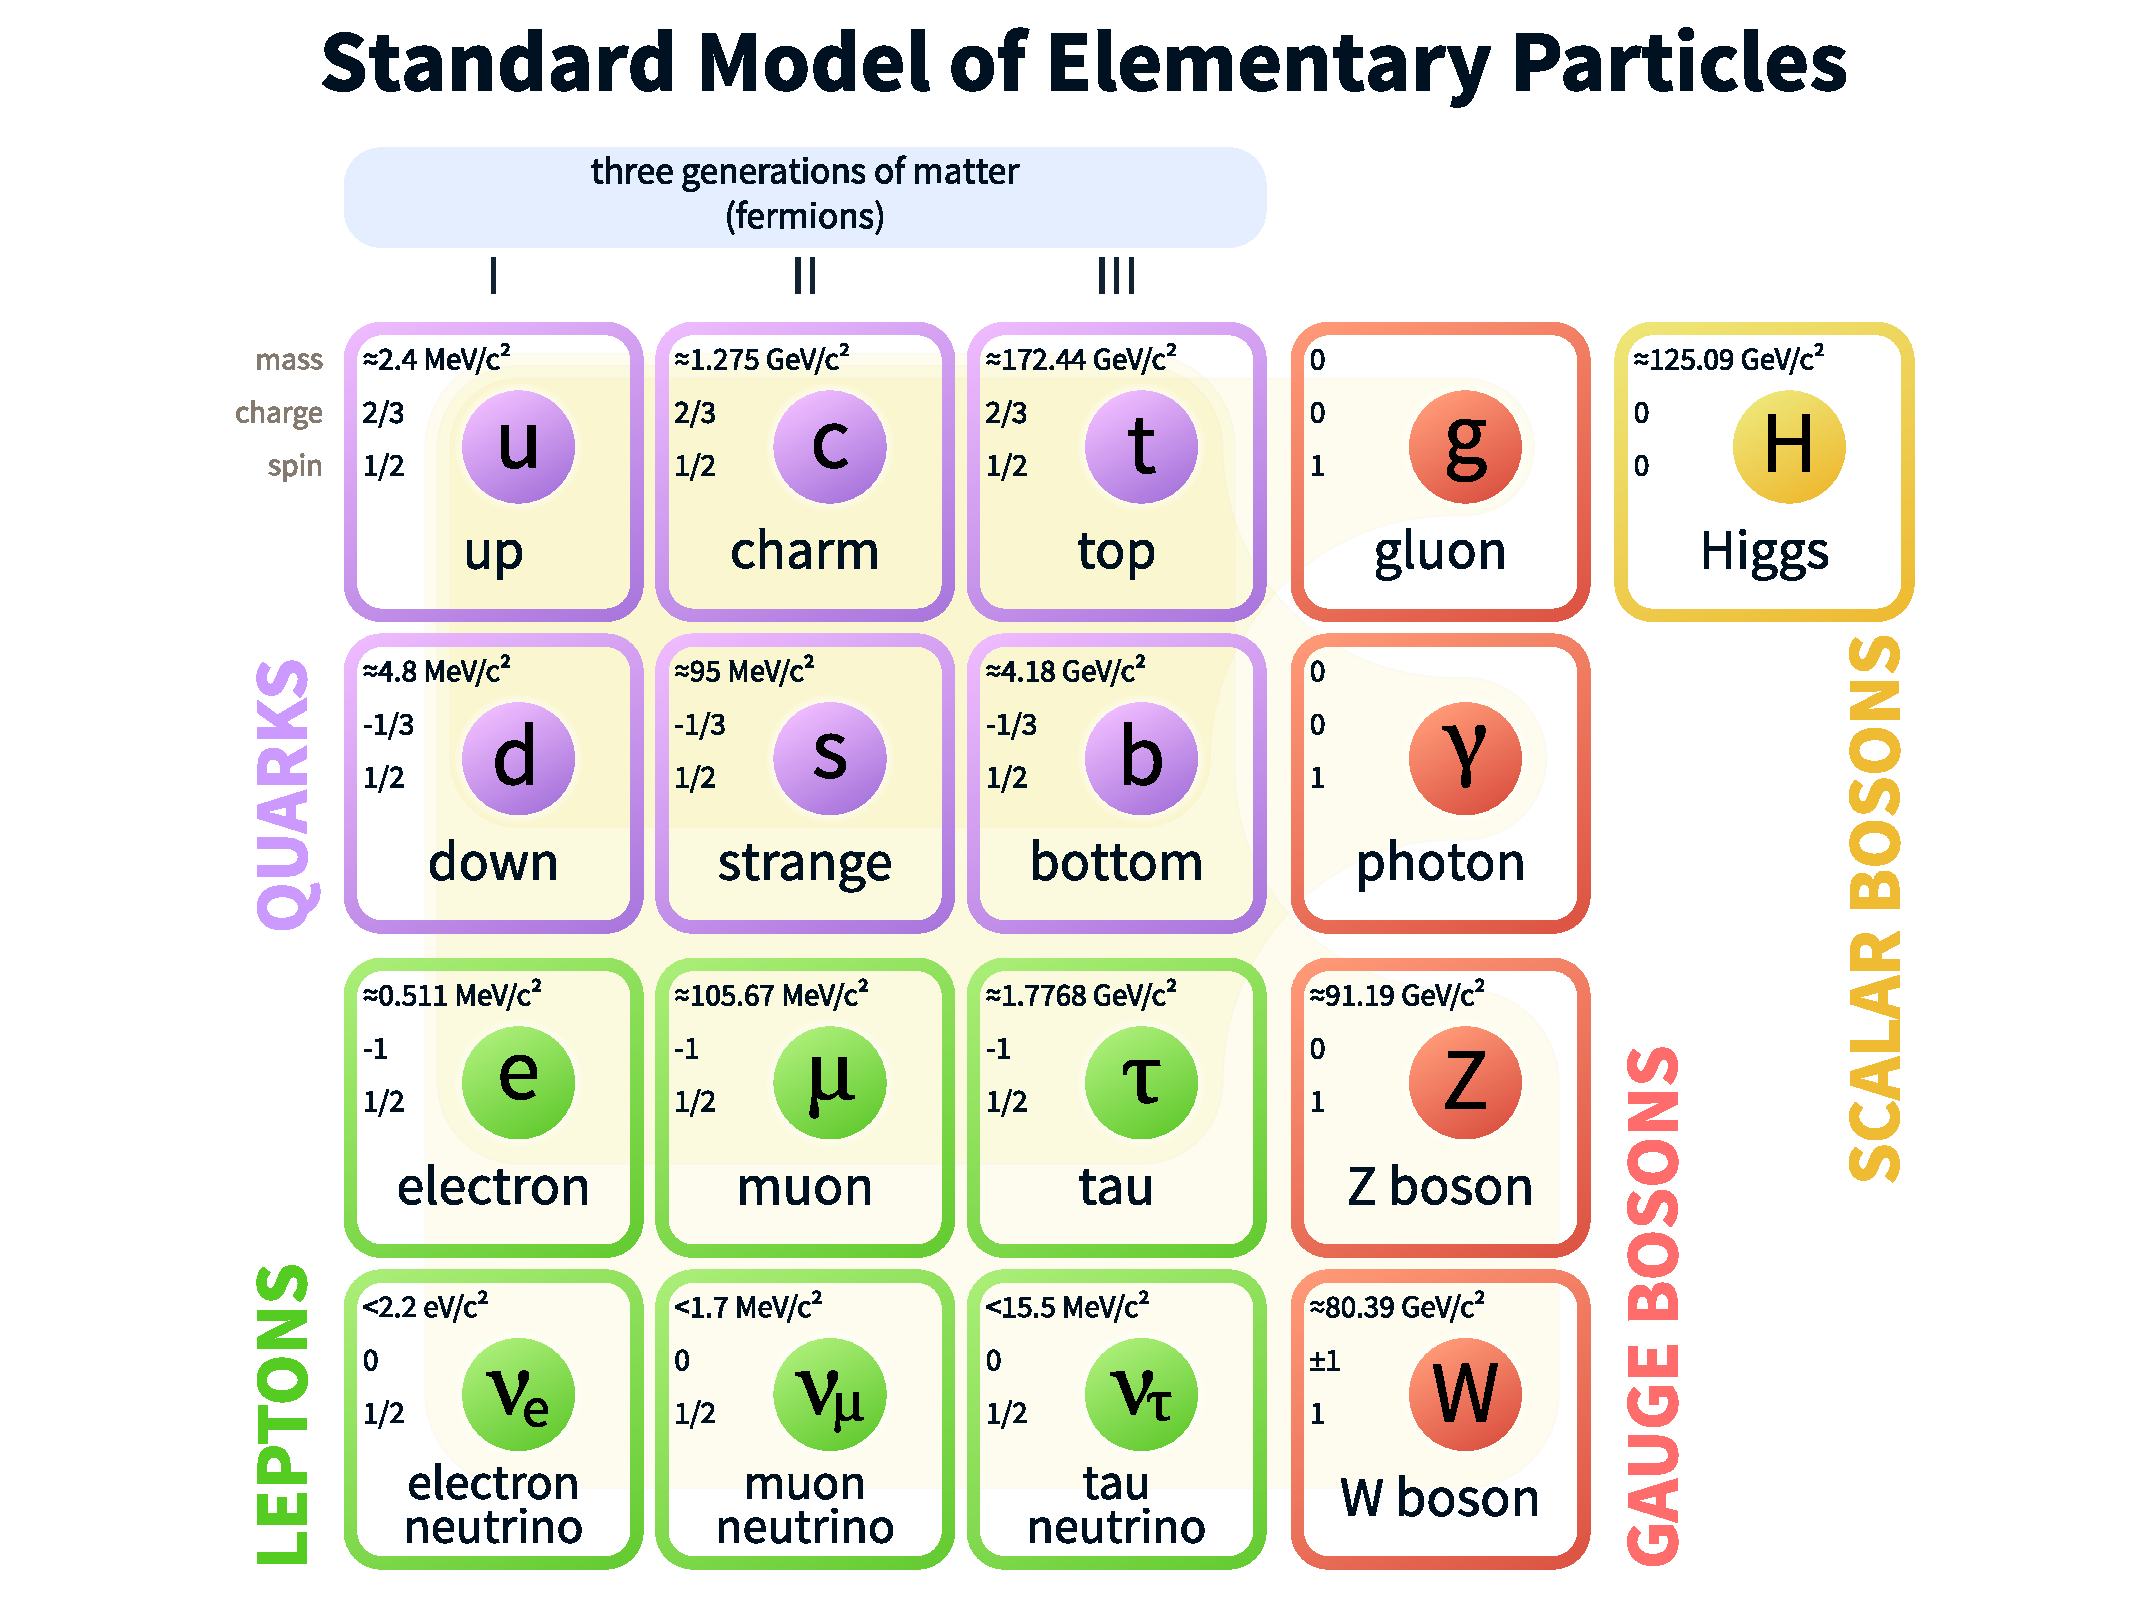
\includegraphics[width=0.72\linewidth]{figures/smpfamily.pdf}
\caption{The Standard Model contains 3 generations' leptons and quarks, 4 kinds of vector bosons and the Higgs boson.}
\label{fig:smpfamily}
\end{center}
\end{figure}

\subsection{Fermions}
Fermions are particles that follow Fermi–Dirac statistics and obey the Pauli exclusion principle. Every fermion has its anti particle, which is a fermion with opposite charge but same mass and spin. The elementary fermions in the Standard Model includes leptons and quarks, both of them consist of 3 generations and each generation consists of 2 flavors of fermions. Every elementary fermion in the Standard Model has half spin.
\subsubsection{Lepton}
The leptons are the fermions that never participate in strong interaction. There are 3 generations of leptons, and each generation consists of two flavors of leptons: one charged lepton such as electrons, and one neutral lepton also known as "neutrino". The charged letpon always carries 1 unit of elementary electric charge, negative for a lepton and possitive for its anti-lepton. The charged leptons have their masses and the masses have been precisely measured as shown in Figure~\ref{fig:smpfamily}. In SM, neutrinos are regarded to be massless.

\vspace{0.3cm}
The first generation of leptons includes electron($e^{-}$) and electron-neutrino($\nu _{e}$). Both electron and electron-neutrino have an electron number $L_{e}=1$, while their anti leptons have $L_{e}=-1$. The second generation leptons, including muon($\mu$) and muon-neutrino($\nu_{\mu}$), have a muon number $L_{\mu}=1$, while $L_{\mu }=-1$ for anti-muon($\bar{\mu}$) and anti-muon-neutrino($\bar{\nu} _{\mu }$). Similarly, the third generation consists of tau($\tau$) and tau-neutrino($\nu _{\tau }$), with a tau number $L_{\tau}$ accordingly.

\vspace{0.3cm}
In SM, under the assumption that neutrinos are massless, the lepton numbers are strictly conserved in any kind of interactions. However, recent experiments\cite{neutrinoOscillation1}\cite{neutrinoOscillation2} indicate that the neutrinos have small masses, which implies the lepton numbers can be mixed among different generations,  with small cross-sections though.
\subsubsection{Quark}
A quark can participate in any of the 3 interactions in Standard Model. Like leptons, quarks fall into 3 generations, and each generation contains 2 flavors of quarks which each have 2/3 and -1/3 elementary electric charge correspondingly. Besides electric charge, quarks also have another intrinsic property known as color charge. The color charge a quark carries can be red, blue or green, while the anti quark carries a corresponding anti-color. Quarks are never observed directly in isolated state due to the phenomenon of color confinement, which confines quarks to only exists in composite colorless particles known as hadrons.

\vspace{0.3cm}
The first generation includes up and down quarks, the second generation includes charm and strange quarks, and the third generation consists of top and bottom quarks. Every quark has its anti quark, with opposite charge of itself. The mass for each quark is shown in Figure~\ref{fig:smpfamily}. It is possible for heavier quarks to decay into lighter quarks through weak interaction, especially for quarks within the same generation.
\subsection{Bosons and the interactions}
In contrast to fermions, bosons are particles that follow Bose–Einstein statistics and alows multi particles in the same state. In SM there are 4 kinds of vector bosons each with spin 1 and one spin-0 scalar boson which is the lately discovered Higgs boson. The vector bosons work as force carriers of the 3 interactions, and the Higgs boson deliever masses to elementary particles by interacting with them.
\subsubsection{Vector Bosons}
In SM, the vector bosons work as mediations of the 3 fundamental interactions among fermions, including gluon, photon, Z boson and W boson. Each of the vector bosons has spin 1.
\begin{itemize}
\item \textbf{gluon} is the force mediation of strong interaction, described in Quantum Chromodynamics (QCD) theory, a gauge theory based on SU(3). Gluons are massless and has no electric charge.
\item \textbf{photon} is the force mediation of electromagnetic interaction, described in Quantum Electrodynamics (QED) theory, a $U(1)_{EM}$ theory. Photons are massless and has no electric charge.
\item \textbf{Z boson} is the mediation of weak interaction with no electric charge flow. The Z boson has no charge, while it has mass of 91.2 GeV, which makes it possible to decay into a pair of fermion–antifermion.
\item \textbf{W boson} is the mediation of weak interaction with electric charge flow. The W carries either 1 or -1 elementary electric charge, noted as $W^{+}$ and $W^{1}$, both having mmasses of 80.4 GeV. Like the Z boson, W bosons can decay into fermion–antifermion pairs.
\end{itemize}
In SM, the unification of electromagnetic interaction and weak interaction is realized by an SU(2) $\times$ U(1) gauge group. Photon, Z boson and W boson are the productions of the SU(2) $\times$ U(1) group due to spontaneous symmetry breaking caused by the Higgs mechanism. 
\subsubsection{The Higgs}
In the 1960s, the Higgs boson and Higgs mechanism is proposed in gesture to explain the source of gauge bosons' masses\cite{higgstheory1}\cite{higgstheory2}\cite{higgstheory3}, as the gauge bosons are believed to be massless according to the gauge theory, which conflicts with the experiment facts. It indicates that the massless gauge bosons interact with a scalar field which leads to a spontaneous symmetry breaking and finally gives mass to the gauge bosons. The scalar field here is the Higgs field. 

\vspace{0.3cm}
On July 4 of 2012, the god particle Higgs boson was announced to be discovered by both CMS and ATLAS experiments at LHC, CERN\cite{higgsdiscover1}\cite{higgsdiscover2}. Hence the Higgs boson officially became one member of the standard model elementary particle family. The Higgs boson has no spin or electric charge, and its mass is measured to be 125GeV. It is very unstable and mainly decays into b$\bar{b}$ quark pair, $\tau\bar{\tau}$ pairs or gauge boson pairs.

\section{The Limit of Standard Model}


\section{Bulk RS Graviton Model and extra dimension}



